\section{Method}
\label{sec:method}

\begin{figure*}[t]
\centering
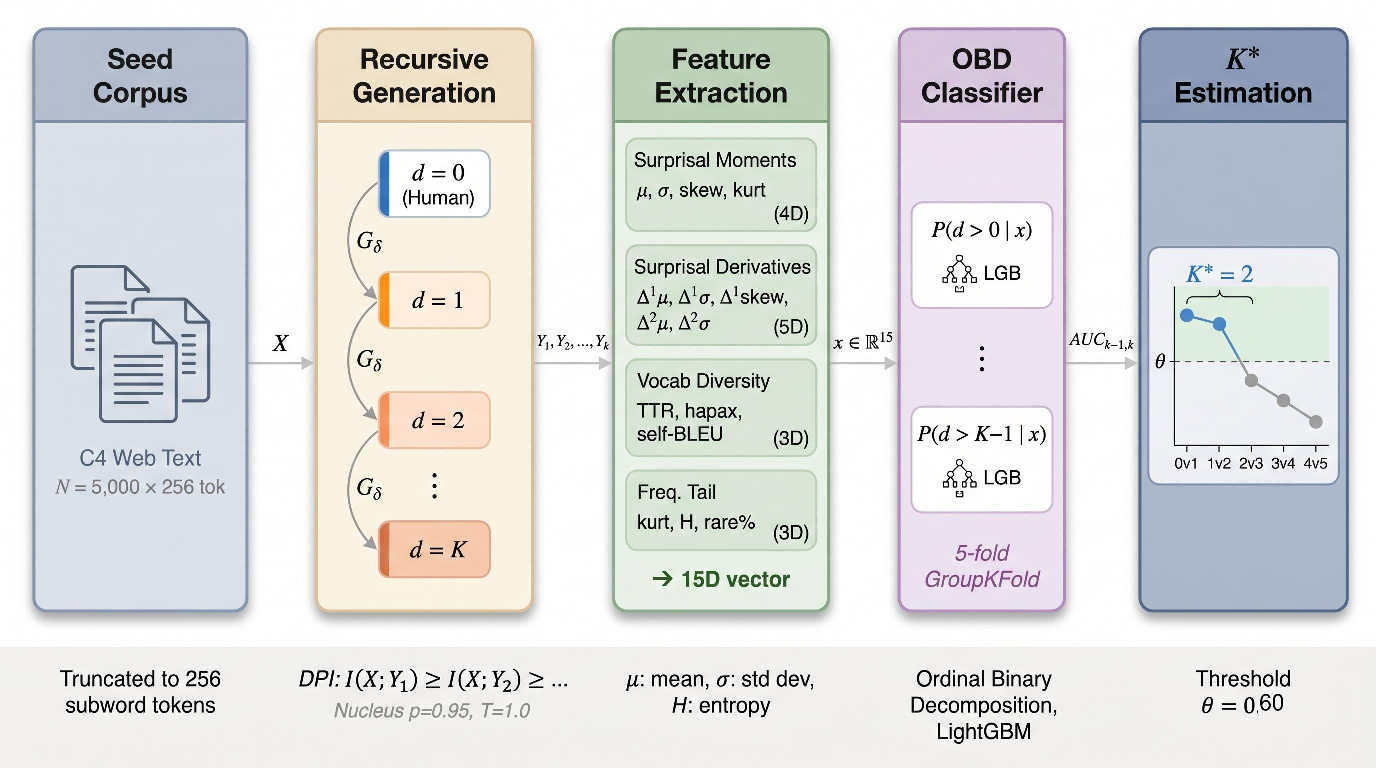
\includegraphics[width=\textwidth]{figures/pipeline.pdf}
\caption{Generational depth estimation pipeline. Seed documents are recursively passed through a generation operator $G_\delta$ to produce a depth chain. Corpus-level statistical features are fed to the OBD-LightGBM classifier for depth prediction. (Simplified notation; see Eq.~\ref{eq:kstar} for the formal $\Kempirical$ definition.)}
\label{fig:pipeline}
\end{figure*}

\subsection{Problem Formulation}
\label{sec:formulation}

A generation operator $G_\delta$ (LLM + decoding strategy $\delta$) produces successive generations $X \to Y_1 \to \cdots \to Y_K$, where $Y_k = G_\delta(Y_{k-1})$ and $Y_0 \triangleq X$ (Figure~\ref{fig:pipeline}).
This sequence forms a Markov chain.
By the Data Processing Inequality, $I(X; Y_1) \geq I(X; Y_2) \geq \cdots \geq 0$: mutual information with the seed text degrades monotonically.
Together with Markov chain convergence, this motivates the existence of a finite discrimination boundary where $\auc_{k-1,k}$ falls below a decision threshold, though AUC and mutual information are not formally equivalent; the actual saturation depth must therefore be measured empirically.
Pairwise AUC generally decreases with depth but may exhibit noise-level reversals (e.g., Pythia-1.4B 3v4 $\auc = 0.505$ vs.\ 4v5 $= 0.508$, a difference within bootstrap CI; Table~\ref{tab:kstar_ci_extended}), reinforcing that $\Kempirical$ is a measured quantity rather than a theoretical prediction.

We define the operational lower bound:
{\small
\begin{equation}
  \Kempirical = \max\bigl\{k \!\geq\! 1 : \auc_{j-1,j} > \theta,\;\forall\, 1 \!\leq\! j \!\leq\! k\bigr\},
  \label{eq:kstar}
\end{equation}
}
which requires all pairs up to depth $k$ to exceed the threshold (the $\forall j$ constraint is naturally satisfied because $\auc_{k-1,k}$ decreases monotonically above $\theta$ across all tested configurations; Table~\ref{tab:kstar_ci}).
The theoretical upper bound $\Ktheory$ (the true maximum discriminable depth given optimal features) is not directly estimated in this work.
Since any specific classifier on a feature subset achieves AUC at most equal to the Bayes-optimal classifier on all features, $\Kempirical \leq \Ktheory$ follows directly.
The DPI motivates the empirical observation that $\auc_{k-1,k}$ generally decreases with $k$ under non-degenerate decoding, though AUC is not a monotone function of MI (as noted above).
Here $\auc_{k-1,k}$ is the point-estimate pairwise AUC and $\theta = 0.60$ is a reference operating point; $\theta$ sits between the 1v2 AUC cluster ($0.607$--$0.696$) and the 2v3 cluster ($0.55$--$0.59$), so that $\Kempirical$ is insensitive to the exact threshold within this range (justified below; Figure~\ref{fig:kstar_theta}).
All pairwise significance tests use 10{,}000-iteration permutation tests with Bonferroni correction for 10 comparisons ($\alpha_{\text{corrected}}{=}0.005$); we report bootstrap 95\% confidence intervals (CIs) (1{,}000 resamples unless otherwise noted) for all boundary-pair AUCs and explicitly mark marginal cases where Bonferroni-corrected lower bounds fall below $\theta$ (Section~\ref{sec:kstar_boundary}).

\paragraph{Threshold justification.}
$\theta{=}0.60$ is a reference operating point supported by two independent lines of evidence.
First, a 10{,}000-iteration permutation test yields a 95th-percentile null of ${<}\,0.55$ ($p < 0.002$ for all boundary comparisons).
Second, $\Kempirical{=}2$ is insensitive to the exact threshold: 1v2 AUC values cluster at $0.607$--$0.696$ while 2v3 values cluster at $0.55$--$0.59$, a ${\sim}$1--10\,pp discontinuity that ensures $\Kempirical$ is stable across $\theta \in [0.59, 0.60]$; at $\theta{=}0.61$, one borderline case (Pythia-1.4B, 1v2 $\auc{=}0.607$) shifts to $\Kempirical{=}1$.
Only at extremes does $\Kempirical$ shift broadly ($\theta{=}0.55$: $\Kempirical{=}3$ for two Qwen configurations; $\theta{=}0.70$: $\Kempirical{=}1$ across all).
Figure~\ref{fig:kstar_theta} provides the full sensitivity surface across $\theta \in [0.50, 0.70]$.
The downstream filtering evaluation (Section~\ref{sec:filtering}) uses the OBD classifier without re-optimizing $\theta$, avoiding circularity.

\subsection{Features and Classifier}
\label{sec:features}

Each document is characterized by a 15-dimensional feature vector spanning four groups: \emph{surprisal moments} (mean, std, skewness, kurtosis; 4~dims), \emph{surprisal derivatives} (mean and std of first- and second-order differences, plus first-order skewness; 5~dims), \emph{vocabulary diversity} (type-token ratio (TTR), hapax legomena ratio, self-BLEU; 3~dims), and \emph{frequency tail statistics} (frequency kurtosis, entropy, rare token fraction; 3~dims).
All features are computed from token-level surprisal values via an external scorer model (full definitions in Table~\ref{tab:s5_features}, Appendix).
Self-BLEU reference sets are drawn exclusively within each fold to prevent information leakage across cross-validation splits; self-BLEU ranks \#1 in 1/8 conditions (greedy decoding) but is absent from the top-3 in all 7 others.
Removing self-BLEU reduces mean $\auc_{1v2}$ by $< 1$\,pp across all models (14D $\Kempirical = 2$ for all 4 configurations); in deployment where reference corpora are unavailable, self-BLEU can be replaced with corpus-level self-similarity or omitted entirely, leaving 14 features (surprisal statistics, TTR, hapax ratio, frequency tail) that require no external reference and retain full $\Kempirical$.
These features are generator-agnostic in that they require no knowledge of or access to the generating model, though they depend on an external scorer for surprisal computation (Section~\ref{sec:transfer}).

We use \emph{Ordinal Binary Decomposition} (OBD), decomposing the $(K{+}1)$-class problem into $K$ cumulative binary sub-classifiers, each estimating $P(\text{depth} > k \mid \mathbf{x})$ via LightGBM (hyperparameters in Table~\ref{tab:s6_lgbm_params}).
OBD achieves lower mean absolute error (MAE) than multiclass LightGBM (e.g., 0.984 vs.\ 1.016 on Qwen-rewrite) while maintaining superior pairwise $\auc$ (mean 0.6095 vs.\ 0.4883 for ordinal logistic regression) (Appendix~\ref{sec:computation_cost}).

\subsection{Experimental Setup}
\label{sec:experimental_setup}

We evaluate six primary configurations spanning three model families (Table~\ref{tab:setup}): Qwen2.5-1.5B-Instruct (rewrite and continuation), Qwen2.5-1.5B (base), Qwen2.5-7B, Pythia-1.4B, and OLMo-1B; four additional models are introduced in Section~\ref{sec:experiments}.
Each uses 5{,}000 C4 seeds truncated to 256 tokens, recursively generated for $K{=}5$ iterations (30{,}000 documents per configuration; Table~\ref{tab:s4_dataset_stats}).
Default decoding: nucleus $p{=}0.95$, $T{=}1.0$; decoding ablation covers greedy, nucleus $p{=}0.9$, $T{=}0.7$, and $T{=}1.2$.
Continuation mode truncates seeds to 128 tokens and extends to 256; rewrite mode paraphrases the full text.
Evaluation: 5-fold GroupKFold cross-validation grouped by seed document; pairwise $\auc$ as primary metric.

\begin{table}[t]
\centering
\small
\caption{Experimental configurations for depth-chain generation. \textbf{Config}: shorthand identifier; \textbf{Model}: architecture and parameter count; \textbf{Mode}: generation strategy (continuation or rewrite); $N$: number of seed documents per depth level.}
\label{tab:setup}
\begin{tabular}{llcc}
\toprule
\textbf{Config} & \textbf{Model} & \textbf{Mode} & $N$ \\
\midrule
Qwen-rw   & Qwen2.5-1.5B-Instruct & Rewrite & 5{,}000 \\
Qwen-cont & Qwen2.5-1.5B-Instruct & Continuation & 5{,}000 \\
Qwen-base & Qwen2.5-1.5B          & Continuation & 5{,}000 \\
Pythia    & Pythia-1.4B            & Continuation & 5{,}000 \\
OLMo      & OLMo-1B               & Continuation & 5{,}000 \\
Qwen-7B   & Qwen2.5-7B            & Continuation & 5{,}000 \\
\bottomrule
\end{tabular}
\end{table}
